\def\figureRandFrame{

\begin{figure}
    \centering

\scriptsize{
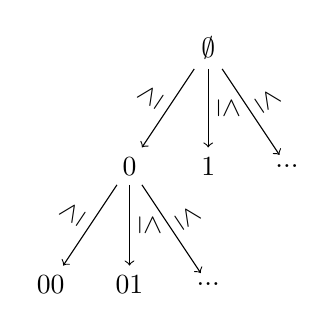
\begin{tikzpicture}
            % Root node
            \node (root) at (0,0) {$\emptyset$};
        
            % Second stage nodes
            \node (n1) at (-1,-1.5) {$0$};
            \node (n2) at (0,-1.5) {$1$};
            \node (n3) at (1,-1.5) {$...$};
        
            % Edges
            \draw[->] (root) -- (n1) node[midway, sloped, above] {$\geq$};
            \draw[->] (root) -- (n2) node[midway, sloped, above] {$\leq$};
            \draw[->] (root) -- (n3) node[midway, sloped, above] {$\leq$};
            
            % Third stage nodes
            \node (n00) at (-2,-3) {$00$};
            \node (n01) at (-1,-3) {$01$};
            \node (n02) at (0,-3) {$...$};
        
            % Edges
            \draw[->] (n1) -- (n00) node[midway, sloped, above] {$\geq$};
            \draw[->] (n1) -- (n01) node[midway, sloped, above] {$\leq$};
            \draw[->] (n1) -- (n02) node[midway, sloped, above] {$\leq$};
        
        \end{tikzpicture}
        \hspace{30pt}
        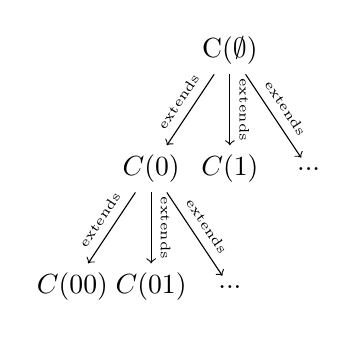
\begin{tikzpicture}
            % Root node
            \node (root) at (0,0) {C($\emptyset$)};
        
            % Second stage nodes
            \node (n1) at (-1,-1.5) {$C(0)$};
            \node (n2) at (0,-1.5) {$C(1)$};
            \node (n3) at (1,-1.5) {$...$};
        
            % Edges
            \draw[->] (root) -- (n1) node[midway, sloped, above] {\tiny{extends}};
            \draw[->] (root) -- (n2) node[midway, sloped, above] {\tiny{extends}};
            \draw[->] (root) -- (n3) node[midway, sloped, above] {\tiny{extends}};
            
            % Third stage nodes
            \node (n00) at (-2,-3) {$C(00)$};
            \node (n01) at (-1,-3) {$C(01)$};
            \node (n02) at (0,-3) {$...$};
        
            % Edges
            \draw[->] (n1) -- (n00) node[midway, sloped, above] {\tiny{extends}};
            \draw[->] (n1) -- (n01) node[midway, sloped, above] {\tiny{extends}};
            \draw[->] (n1) -- (n02) node[midway, sloped, above] {\tiny{extends}};

        \end{tikzpicture}
  

}

    \caption{R and a Kripke frame }
    \label{fig:enter-label}
    
\end{figure}
}

\def\tableauxCumulativeAndNonCumulativeExampleFigure{
    \begin{figure}
        \centering
        \scriptsize{
        \makebox[\textwidth][c]{%
        \resizebox{1\textwidth}{!}{
        \begin{tikzpicture}
            % Root node
            \node (root) at (0,0) {$F_{\emptyset} \alpha \to \neg \neg \alpha$};
            
            % Second stage nodes
            \node (n1) at (0,-1.5) {$T_{0} \alpha$};
            \draw[->] (root) -- (n1);
            
            % Third stage nodes
            \node (n2) at (0,-3) {$F_{0} \neg \neg \alpha$};
            \draw[->] (n1) -- (n2);
            
            % Fourth stage nodes
            \node (n3) at (0,-4.5) {$T_{00} \neg \alpha$};
            \draw[->] (n2) -- (n3);

            
            % Fifth stage nodes
            \node (n4) at (0,-6) {$F_{00} \alpha$};
            \draw[->] (n3) -- (n4);

            \node (n5) at (0,-7.5) {X};
            \draw[->] (n4) -- (n5);
        \end{tikzpicture}

        \hspace{1cm}

        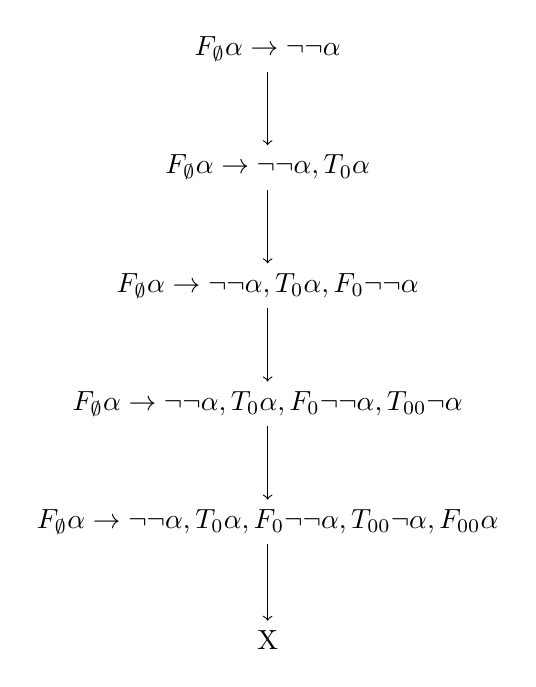
\begin{tikzpicture}
            % Root node
            \node (root) at (0,0) {$F_{\emptyset} \alpha \to \neg \neg \alpha$};
            
            % Second stage nodes
            \node (n1) at (0,-1.5) {$F_{\emptyset} \alpha \to \neg \neg \alpha, T_{0} \alpha$};
            \draw[->] (root) -- (n1);
            
            % Third stage nodes
            \node (n2) at (0,-3) {$F_{\emptyset} \alpha \to \neg \neg \alpha, T_{0} \alpha, F_{0} \neg \neg \alpha$};
            \draw[->] (n1) -- (n2);
            
            % Fourth stage nodes
            \node (n3) at (0,-4.5) {$F_{\emptyset} \alpha \to \neg \neg \alpha, T_{0} \alpha, F_{0} \neg \neg \alpha, T_{00} \neg \alpha$};
            \draw[->] (n2) -- (n3);
            
            % Fifth stage nodes
            \node (n4) at (0,-6) {$F_{\emptyset} \alpha \to \neg \neg \alpha, T_{0} \alpha, F_{0} \neg \neg \alpha, T_{00} \neg \alpha, F_{00} \alpha$};
            \draw[->] (n3) -- (n4);

            \node (n5) at (0,-7.5) {X};
            \draw[->] (n4) -- (n5);
        \end{tikzpicture}

        \hspace{1cm}

        \begin{tikzpicture}
            % Root node
            \node (root) at (0,0) {$F_{\emptyset} \alpha \to \neg \neg \alpha$};
            
            % Second stage nodes
            
            % Third stage nodes
            \node (n2) at (0,-3) {$F_{\emptyset} \alpha \to \neg \neg \alpha, T_{0} \alpha, F_{0} \neg \neg \alpha$};
            \draw[->] (root) -- (n2);
            
            % Fourth stage nodes
            \node (n3) at (0,-4.5) {$F_{\emptyset} \alpha \to \neg \neg \alpha, T_{0} \alpha, F_{0} \neg \neg \alpha, T_{00} \neg \alpha$};
            \draw[->] (n2) -- (n3);
            
            % Fifth stage nodes
            \node (n4) at (0,-6) {$F_{\emptyset} \alpha \to \neg \neg \alpha, T_{0} \alpha, F_{0} \neg \neg \alpha, T_{00} \neg \alpha, F_{00} \alpha$};
            \draw[->] (n3) -- (n4);

            \node (n5) at (0,-7.5) {X};
            \draw[->] (n4) -- (n5);
        \end{tikzpicture}
        }
        }
        }
        \caption{Example of a destructive tableaux proof tree from \cite{book1}, the intermediary structure and the non-destructive tableaux proof tree.}
        \label{fig:destructive_tableaux}
    \end{figure}
}


